%%%%%%%%%%%%%%%%%%%%%%%%%%%%%%%%%%%%
% Slide options
%%%%%%%%%%%%%%%%%%%%%%%%%%%%%%%%%%%%

% Option 1: Slides with solutions

\documentclass[slidestop,compress,mathserif]{beamer}
\newcommand{\soln}[1]{\textit{#1}}
\newcommand{\solnGr}[1]{#1}

% Option 2: Handouts without solutions

%\documentclass[11pt,containsverbatim,handout]{beamer}
%\usepackage{pgfpages}
%\pgfpagesuselayout{4 on 1}[letterpaper,landscape,border shrink=5mm]
%\newcommand{\soln}[1]{ }
%\newcommand{\solnGr}{ }


%%%%%%%%%%%%%%%%%%%%%%%%%%%%%%%%%%%%
% Style
%%%%%%%%%%%%%%%%%%%%%%%%%%%%%%%%%%%%

\def\chpiv@path{../../Chp 4}
\input{../../lec_style.tex}

%%%%%%%%%%%%%%%%%%%%%%%%%%%%%%%%%%%%
% Preamble
%%%%%%%%%%%%%%%%%%%%%%%%%%%%%%%%%%%%

\title[Lecture 12]{MA213: Lecture 12}
\subtitle{Module 2: Probability, Random Variables, and Distributions}
\author{OpenIntro Statistics, 4th Edition}
\institute{$\:$ \\ {\footnotesize Based on slides developed by Mine \c{C}etinkaya-Rundel of OpenIntro. \\
The slides may be copied, edited, and/or shared via the \webLink{http://creativecommons.org/licenses/by-sa/3.0/us/}{CC BY-SA license.} \\
Some images may be included under fair use guidelines (educational purposes).}}
\date{}

%%%%%%%%%%%%%%%%%%%%%%%%%%%%%%%%%%%%
% Begin document
%%%%%%%%%%%%%%%%%%%%%%%%%%%%%%%%%%%%

\begin{document}


%%%%%%%%%%%%%%%%%%%%%%%%%%%%%%%%%%%%
% Title page
%%%%%%%%%%%%%%%%%%%%%%%%%%%%%%%%%%%%

{
\addtocounter{framenumber}{-1} 
{\removepagenumbers 
\usebackgroundtemplate{\includegraphics[width=\paperwidth]{../../OpenIntro_Grid_4_3-01.jpg}}
\begin{frame}

\hfill \includegraphics[width=20mm]{../../oiLogo_highres}

\titlepage

\end{frame}
}
}


%%%%%%%%%%%%%%%%%%%%%%%%%%%%%%%%%%%%
% Recap/Agenda 
%%%%%%%%%%%%%%%%%%%%%%%%%%%%%%%%%%%%
% TODO better formatting
\begin{frame}
    \frametitle{Module 2: Probability, Random Variables, and Distributions}
    \begin{itemize}
        \item \hl{Previously: } Normal distribution (Chapter 4.1)
        \item \hl{This time: } Geometric distribution (Chapter 4.2)
        \item \hl{Reading: } Chapter 4.3 for next time
        \item \hl{Deadlines/Announcements: } 
        \begin{enumerate}
            \item HW 4 due today
            \item Quiz 1 retake qualifications due Friday (last appointments on Thursday 9-10am)
            \item Lab groups are on Blackboard (messages, deliverable materials)
            \item Project 1 deliverable 1 due Thurs 10pm
        \end{enumerate}
    \end{itemize}
    
\end{frame}
    
%%%%%%%%%%%%%%%%%%%%%%%%%%%%%%%%%%%%
% Learning objectives:
%%%%%%%%%%%%%%%%%%%%%%%%%%%%%%%%%%%%
\begin{frame}
    \frametitle{Learning Objectives}
    \begin{itemize}
        \item \textbf{M2 LO1: Validate and Explain Probability Distributions:} Assess the validity of a probability distribution using the concepts of outcome, sample space, and probability properties (e.g., disjoint outcomes, probabilities between 0 and 1, and total probabilities summing to 1).
        \item \textbf{M2 LO4: Understand and Compute Expectations and Variances:} Explain the concepts of expectations and variances of random variables, and compute the expectation and variance of a linear combination of random variables.
        \item \textbf{M2 LO5: Model Data Using Bernoulli, Geometric, and Binomial Distributions:} Recognize when to appropriately model data using the Bernoulli, geometric, and binomial distributions, and compute quantities of interest such as mean, standard deviation, and tail probabilities.
    \end{itemize}
\end{frame}


%%%%%%%%%%%%%%%%%%%%%%%%%%%%%%%%%%%%
% Sections
%%%%%%%%%%%%%%%%%%%%%%%%%%%%%%%%%%%%
\section{Normal distribution (cont.)}

\subsection{68-95-99.7 rule}

%%%%%%%%%%%%%%%%%%%%%%%%%%%%%%%%%%%%

\begin{frame}
\frametitle{68-95-99.7 Rule}

\begin{itemize}

\item For nearly normally distributed data, 
\begin{itemize}
\item about 68\% falls within 1 SD of the mean,
\item about 95\% falls within 2 SD of the mean,
\item about 99.7\% falls within 3 SD of the mean.
\end{itemize}

\item It is possible for observations to fall 4, 5, or more standard deviations away from the mean, but these occurrences are very rare if the data are nearly normal.

\end{itemize}

\begin{center}
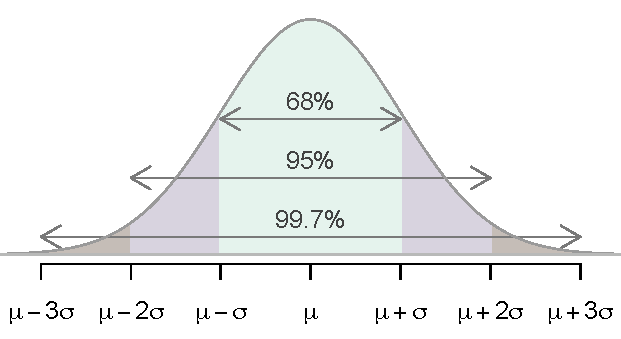
\includegraphics[width=0.7\textwidth]{\chpiv@path/4-1_normal_distribution/figures/6895997/6895997}
\end{center}

\end{frame}

%%%%%%%%%%%%%%%%%%%%%%%%%%%%%%%%%%%%

\begin{frame}
\frametitle{Describing variability using the 68-95-99.7 Rule}

SAT scores are distributed nearly normally with mean 1500 and standard deviation 300.

\pause
\begin{itemize}

\item $\sim$68\% of students score between 1200 and 1800 on the SAT. 

\item $\sim$95\% of students score between 900 and 2100 on the SAT. 

\item $\sim$99.7\% of students score between 600 and 2400 on the SAT. 

\end{itemize}

\begin{center}
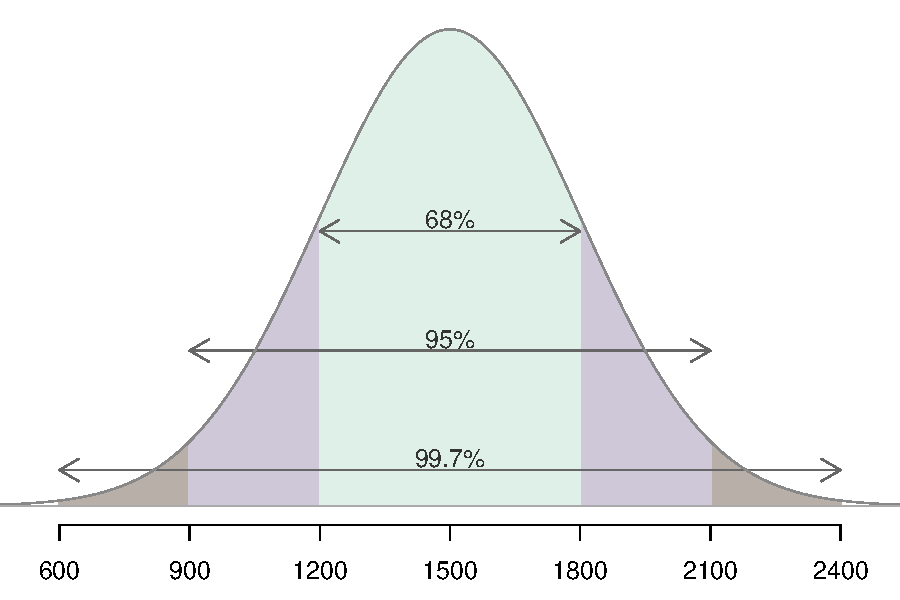
\includegraphics[width=0.65\textwidth]{\chpiv@path/4-1_normal_distribution/figures/sat_empirical/sat_empirical}
\end{center}

\end{frame}

%%%%%%%%%%%%%%%%%%%%%%%%%%%%%%%%%%%%

\section{Edfinity quiz: Geometric logic}  

%%%%%%%%%%%%%%%%%%%%%%%%%%%%%%%%%%%%

\begin{frame}[fragile]
\frametitle{Number of hours of sleep on school nights}

\only<1 | handout:0>{
\begin{center}
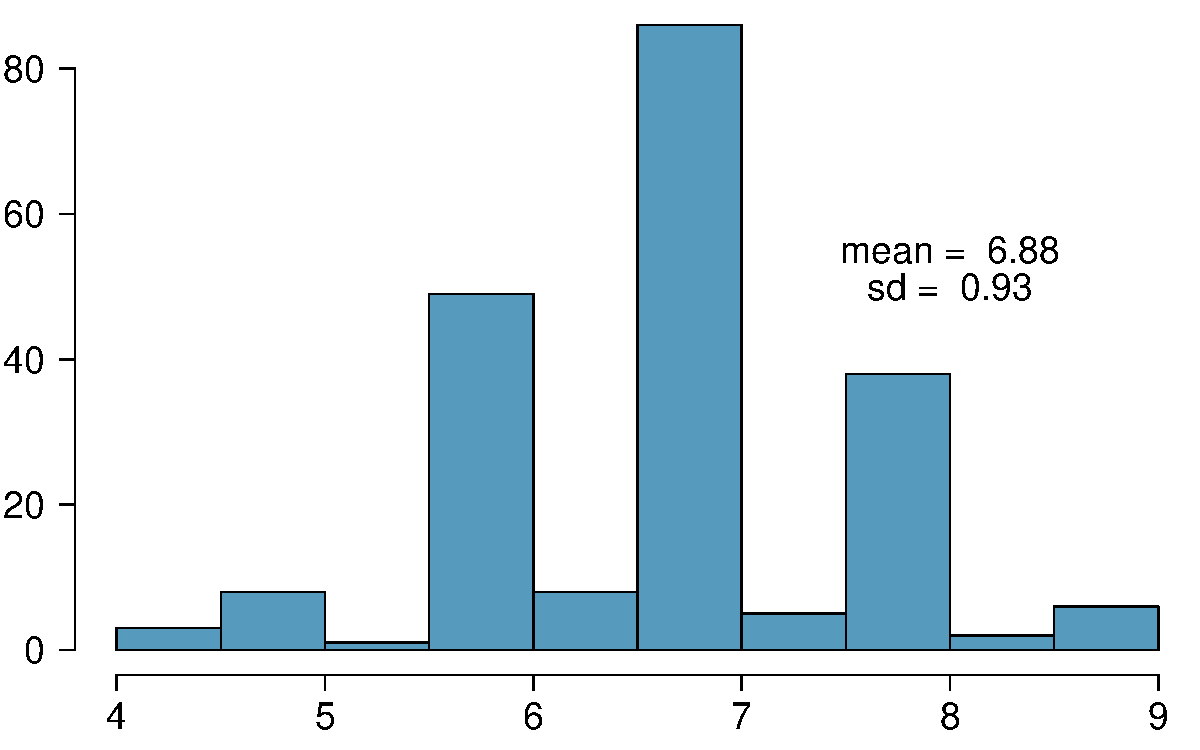
\includegraphics[width=0.75\textwidth]{\chpiv@path/4-1_normal_distribution/figures/sleep/sleep-hist} 
\end{center}
\vspace{-0.25cm}
\begin{itemize}
\item Mean = 6.88 hours, SD = 0.92 hrs
\item[] \textcolor{white}{72\% of the data are within 1 SD of the mean: $6.88 \pm 0.93$}
\item[] \textcolor{white}{92\% of the data are within 2 SD of the mean: $6.88 \pm 2 \times 0.93$}
\item[] \textcolor{white}{99\% of the data are within 3 SD of the mean: $6.88 \pm 3 \times 0.93$}
\end{itemize}
}

\only<2 | handout:0>{
\begin{center}
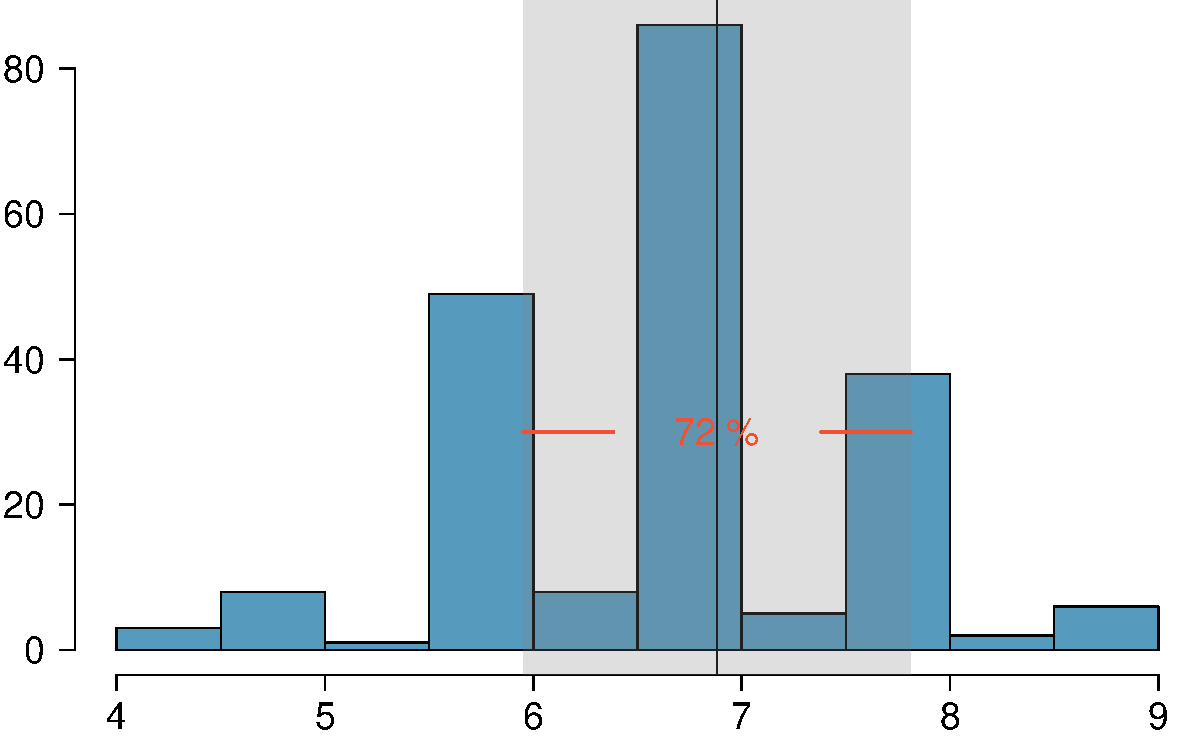
\includegraphics[width=0.75\textwidth]{\chpiv@path/4-1_normal_distribution/figures/sleep/sleep-hist-sd1} 
\end{center}
\vspace{-0.25cm}
\begin{itemize}
\item Mean = 6.88 hours, SD = 0.92 hrs
\item 72\% of the data are within 1 SD of the mean: $6.88 \pm 0.93$
\item[] \textcolor{white}{92\% of the data are within 2 SD of the mean: $6.88 \pm 2 \times 0.93$}
\item[] \textcolor{white}{99\% of the data are within 3 SD of the mean: $6.88 \pm 3 \times 0.93$}
\end{itemize}
}

\only<3 | handout:0>{
\begin{center}
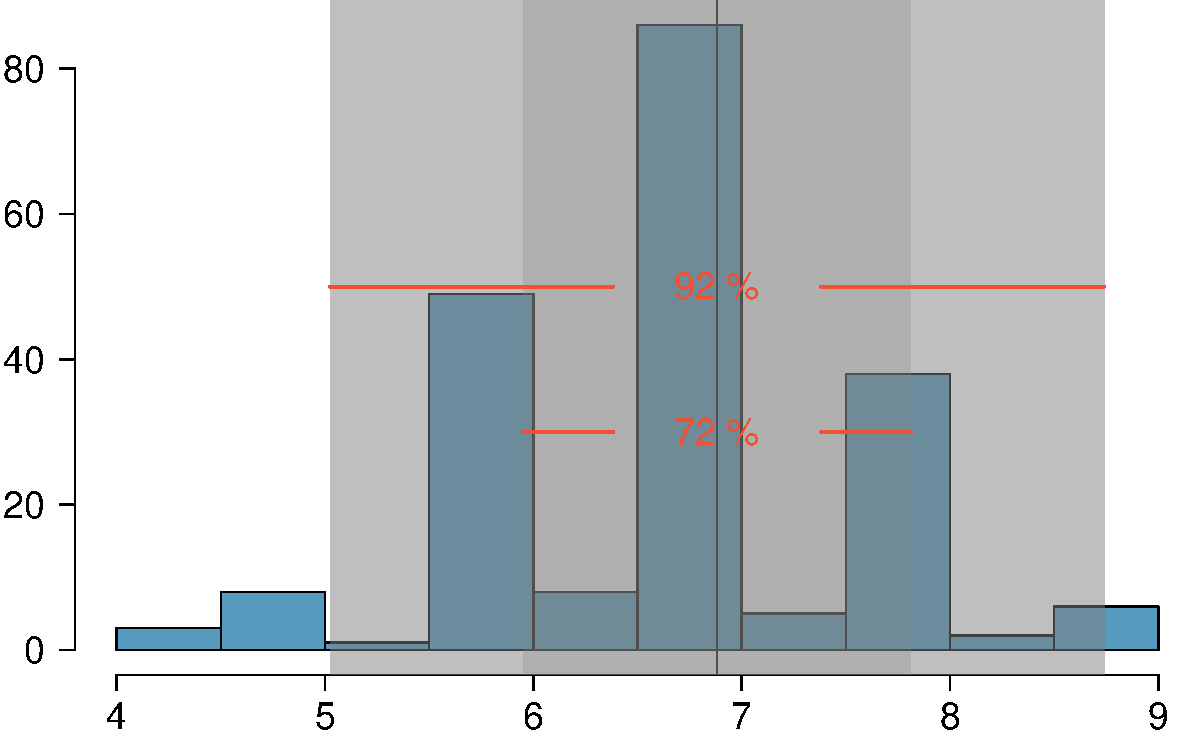
\includegraphics[width=0.75\textwidth]{\chpiv@path/4-1_normal_distribution/figures/sleep/sleep-hist-sd2} 
\end{center}
\vspace{-0.25cm}
\begin{itemize}
\item Mean = 6.88 hours, SD = 0.92 hrs
\item 72\% of the data are within 1 SD of the mean: $6.88 \pm 0.93$
\item 92\% of the data are within 1 SD of the mean: $6.88 \pm 2 \times 0.93$
\item[] \textcolor{white}{99\% of the data are within 3 SD of the mean: $6.88 \pm 3 \times 0.93$}
\end{itemize}
}

\only<4>{
\begin{center}
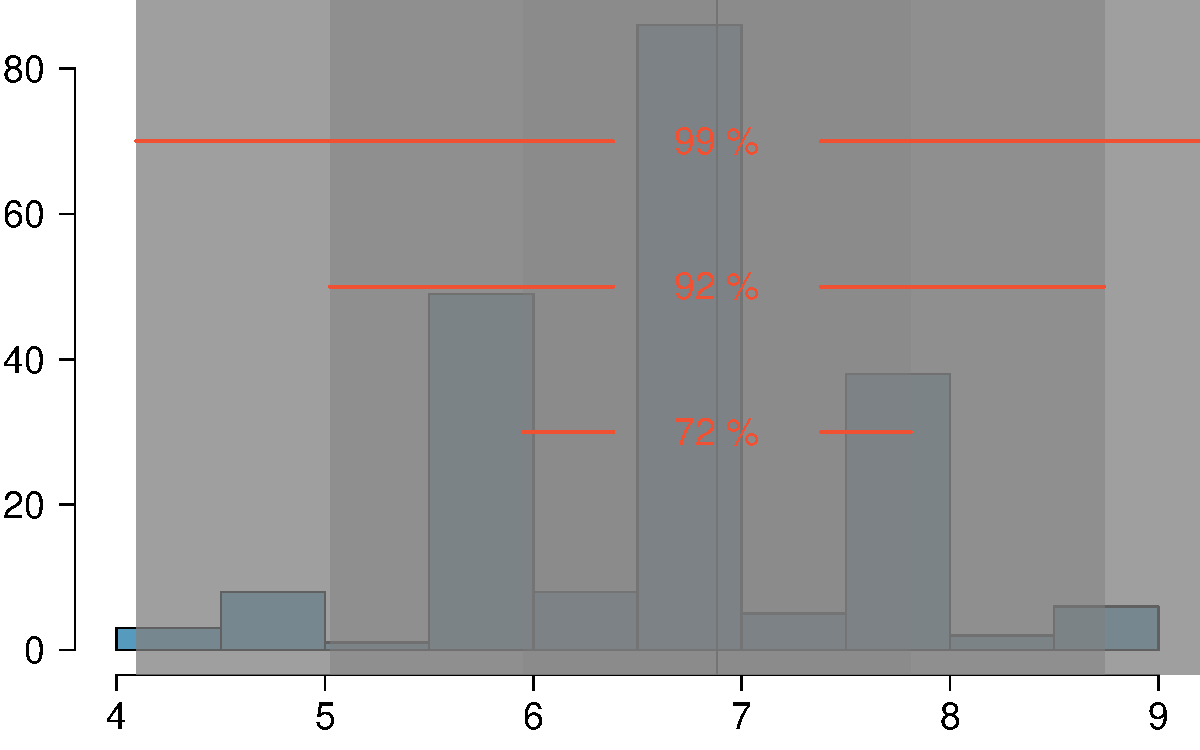
\includegraphics[width=0.75\textwidth]{\chpiv@path/4-1_normal_distribution/figures/sleep/sleep-hist-sd3} 
\end{center}
\vspace{-0.25cm}
\begin{itemize}
\item Mean = 6.88 hours, SD = 0.92 hrs
\item 72\% of the data are within 1 SD of the mean: $6.88 \pm 0.93$
\item 92\% of the data are within 2 SD of the mean: $6.88 \pm 2 \times 0.93$
\item 99\% of the data are within 3 SD of the mean: $6.88 \pm 3 \times 0.93$
\end{itemize}
}

\end{frame}

%%%%%%%%%%%%%%%%%%%%%%%%%%%%%%%%%%%%

\section{Geometric distribution}

%%%%%%%%%%%%%%%%%%%%%%%%%%%%%%%%%%%%

\subsection{Bernoulli distribution}

%%%%%%%%%%%%%%%%%%%%%%%%%%%%%%%%%%%%

\begin{frame}
\frametitle{Milgram experiment}

\twocol{0.65}{0.35}{

\begin{itemize}

\item Stanley Milgram, a Yale University psychologist, conducted a series of experiments on obedience to authority starting in 1963. 

\item Experimenter (E) orders the teacher (T), the subject of the experiment, to give severe electric shocks to a learner (L) each time the learner answers a question incorrectly. 

\item The learner is actually an actor, and the electric shocks are not real, but a prerecorded sound is played each time the teacher administers an electric shock.

\end{itemize}

}
{
\begin{center}
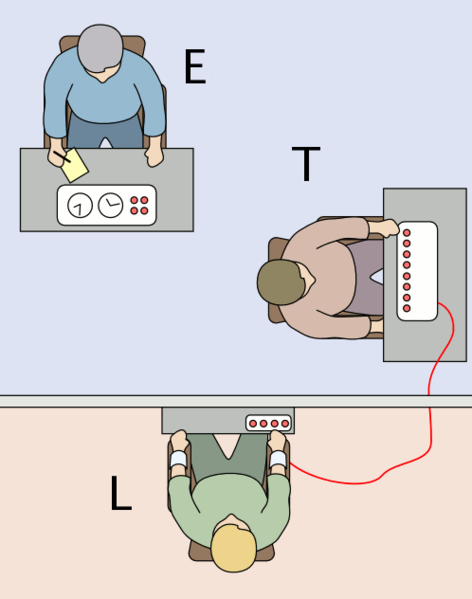
\includegraphics[width=\textwidth]{\chpiv@path/4-2_geometric_distribution/figures/milgram}
\end{center}
\ct{\webURL{http://en.wikipedia.org/wiki/File:Milgram_Experiment_v2.png}}
}

\end{frame}

%%%%%%%%%%%%%%%%%%%%%%%%%%%%%%%%%%%%

\begin{frame}
\frametitle{Milgram experiment (cont.)}

\begin{itemize}

\item These experiments measured the willingness of study participants to obey an authority figure who instructed them to perform acts that conflicted with their personal conscience.

\item Milgram found that about 65\% of people would obey authority and give such shocks.

\item Over the years, additional research suggested this number is approximately consistent across communities and time.

\end{itemize}

\end{frame}


%%%%%%%%%%%%%%%%%%%%%%%%%%%%%%%%%%%%

\begin{frame}
\frametitle{Bernoulli random variables}

\begin{itemize}

\item Each person in Milgram's experiment can be thought of as a \hl{trial}.

\item A person is labeled a \hl{success} if she refuses to administer a severe shock, and \hl{failure} if she administers such shock.

\item Since only 35\% of people refused to administer a shock, \hl{probability of success} is \mathhl{p = 0.35}.

\item When an individual trial has only two possible outcomes, it is called a \hl{Bernoulli random variable}.

\end{itemize}

\twocol{0.3}{0.4}{
    \begin{center}
        \begin{align*}
            X &\sim \text{Bernoulli}(p) \\
            Pr(X=x) &= p^x (1-p)^{1-x}, \quad x = 0, 1
        \end{align*}
    \end{center}
}{
    % Bernoulli Distribution PMF Table
    \begin{small}
    \begin{center}
    \renewcommand{\arraystretch}{1.5}
    \begin{tabular}{l | c | c }
    Event      & $X$   & $P(X)$      \\
    \hline
    Success    & $1$   & $p$         \\
    Failure    & $0$   & $1-p$       \\
    \hline
    Total      &       & $1$         
    \end{tabular}
    \end{center}
    \end{small}
}
\end{frame}

%%%%%%%%%%%%%%%%%%%%%%%%%%%%%%%%%%%%

\section{Edfinity Quiz: Bernoulli Random Variables}

%%%%%%%%%%%%%%%%%%%%%%%%%%%%%%%%%%%%

\subsection{Geometric distribution}

%%%%%%%%%%%%%%%%%%%%%%%%%%%%%%%%%%%%

\begin{frame}
\frametitle{Geometric distribution}

{\small

\dq{Dr. Smith wants to repeat Milgram's experiments but she only wants to sample people until she finds someone who will not inflict a severe shock. What is the probability that she stops after the first person?}

\[ P(1^{st}~person~refuses) = 0.35 \]

\pause

\dq{... the third person?}
\[ P(1^{st}~and~2^{nd}~shock,~3^{rd}~refuses) = \slot{S}{0.65} \times \slot{S}{0.65} \times  \slot{R}{0.35} = 0.65^2 \times 0.35 \approx 0.15 \]

\pause

\dq{... the tenth person?}
\soln{
\pause
\[ P(9~shock,~10^{th}~refuses) = \underbrace{\slot{S}{0.65} \times \cdots \times \slot{S}{0.65}}_{9~of~these} \times  \slot{R}{0.35} = 0.65^9 \times 0.35 \approx 0.0072 \]
}
}

\end{frame}

%%%%%%%%%%%%%%%%%%%%%%%%%%%%%%%%%%%%

\begin{frame}
\frametitle{Geometric distribution (cont.)}

\hl{Geometric distribution} describes the waiting time until a success for \hl{independent and identically distributed (iid)} Bernouilli random variables.
\begin{itemize}
\item independence: outcomes of trials don't affect each other
\item identical: the probability of success is the same for each trial
\end{itemize}

$\:$ \\
$\:$ \\

\pause

\formula{Geometric probabilities}{If $p$ represents probability of success, $(1-p)$ represents probability of failure, and $n$ represents number of independent trials \[P(success~on~the~n^{th}~trial) = (1-p)^{n-1} p\]}

\end{frame}

%%%%%%%%%%%%%%%%%%%%%%%%%%%%%%%%%%%%

\begin{frame}
\frametitle{Geometric distribution}
        $X \sim \text{Geometric}(p) \qquad
        Pr(X=n) = (1-p)^{n-1} p, 
        \quad n = 1, 2, 3, \ldots$

\twocol{0.4}{0.6}{
    \begin{center}
        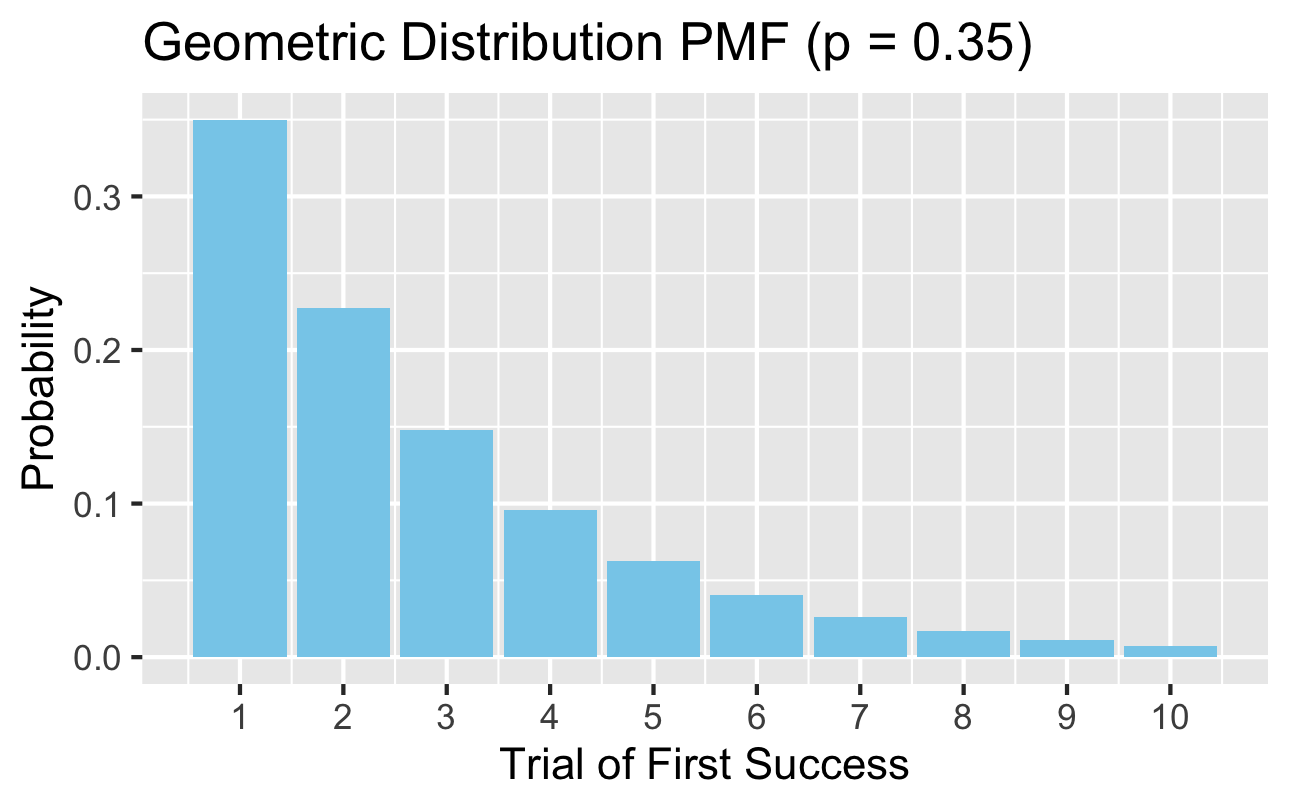
\includegraphics[width=0.35\paperwidth]{figures/geometric_pmf.png}
        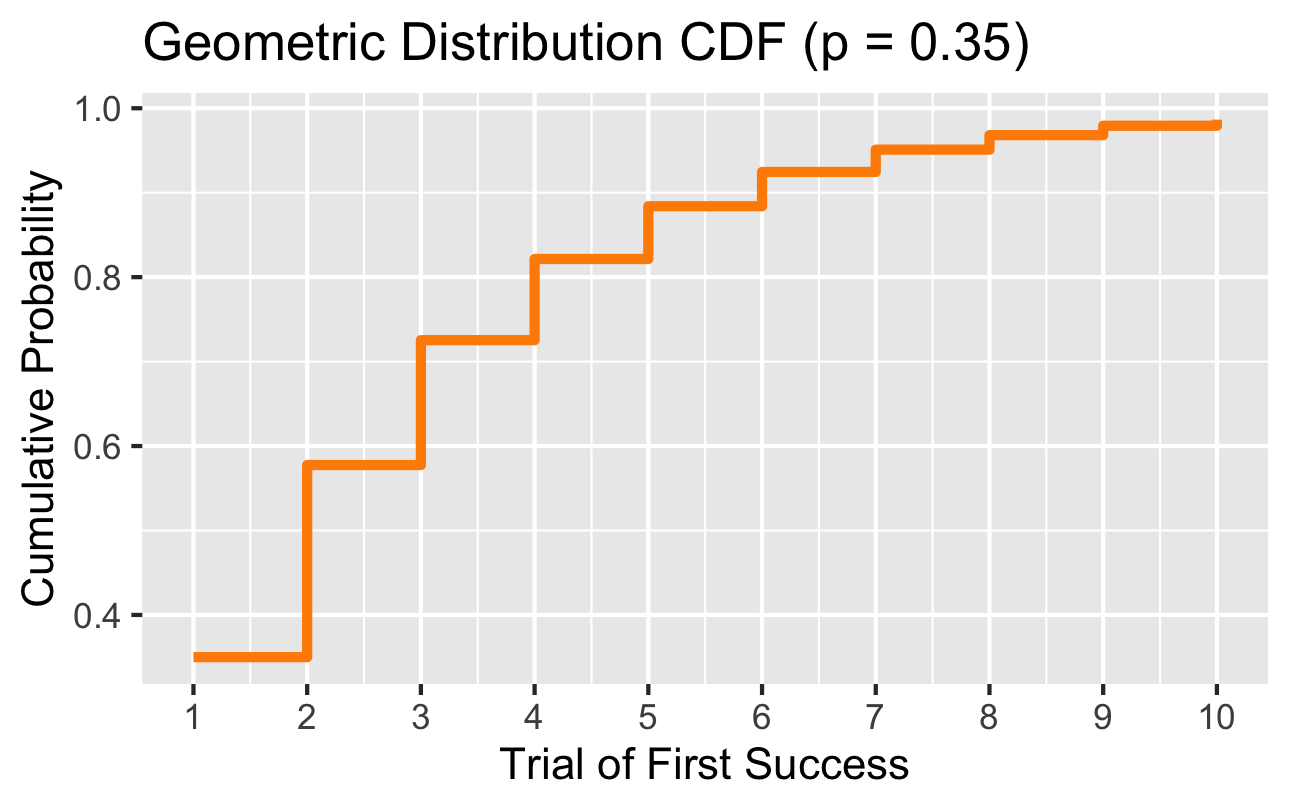
\includegraphics[width=0.35\paperwidth]{figures/geometric_cdf.png}
    \end{center}
}{
    % Geometric Distribution PMF Table
    \begin{small}
    \begin{center}
    \renewcommand{\arraystretch}{1.5}
    \begin{tabular}{l | c | c }
    Event                        & $X$   & $P(X)$              \\
    \hline
    First success on 1st trial   & $1$   & $p$                 \\
    First success on 2nd trial   & $2$   & $(1-p)p$            \\
    First success on 3rd trial   & $3$   & $(1-p)^2 p$         \\
    $\vdots$                     & $\vdots$ & $\vdots$         \\
    First success on $n$th trial & $n$   & $(1-p)^{n-1} p$     \\
    \hline
    Total                        &       & $1$                 \\
    \end{tabular}
    \end{center}
    \end{small}
}

\end{frame}

%%%%%%%%%%%%%%%%%%%%%%%%%%%%%%%%%%%%


%%%%%%%%%%%%%%%%%%%%%%%%%%%%%%%%%%%%

\begin{frame}

\pq{Can we calculate the probability of rolling a 6 for the first time on the 6$^{th}$ roll of a die using the geometric distribution? Note that what was a success (rolling a 6) and what was a failure (not rolling a 6) are clearly defined and one or the other must happen for each trial.}

\begin{enumerate}[(a)]
\item no, on the roll of a die there are more than 2 possible outcomes
\only<1>{\item yes, why not}
\soln{\only<2>{\item \orange{yes, why not}}}
\end{enumerate}

\soln{
\only<2>{
\[P(6~on~the~6^{th}~roll) = \pr{ \frac{5}{6} }^5 \pr{ \frac{1}{6} } \approx 0.067 \]
}
}

\end{frame}


%%%%%%%%%%%%%%%%%%%%%%%%%%%%%%%%%%%%

\section{Edfinity Quiz: Using the Geometric distribution}

%%%%%%%%%%%%%%%%%%%%%%%%%%%%%%%%%%%%

%%%%%%%%%%%%%%%%%%%%%%%%%%%%%%%%%%%%

\begin{frame}
\frametitle{Expected value}

\dq{How many people is Dr. Smith expected to test before finding the first one that refuses to administer the shock?}

\pause

\begin{center}
\renewcommand{\arraystretch}{1.5}
\begin{tabular}{c | c | c }
$X$   & $P(X)$              & $X ~ P(X)$         \\
\hline
$1$   & $p$                 & $1 \times p$       \\
$2$   & $(1-p)p$            & $2 \times (1-p)p$  \\
$3$   & $(1-p)^2 p$         & $3 \times (1-p)^2 p$ \\
$\vdots$   & $\vdots$       & $\vdots$           \\
$n$   & $(1-p)^{n-1} p$     & $n \times (1-p)^{n-1} p$ \\
\hline
      & $1$                 & $E(X) = \sum_{n=1}^{\infty} n (1-p)^{n-1} p \only<3>{=... \textcolor{orange}{= \frac{1}{p}}}$ \\
\end{tabular}
\end{center}
\pause

\textit{This is a complicated infinite sum, so we give you the answer.}

\end{frame}


%%%%%%%%%%%%%%%%%%%%%%%%%%%%%%%%%%%%

\begin{frame}
\frametitle{Expected value}

\dq{How many people is Dr. Smith expected to test before finding the first one that refuses to administer the shock?}

The expected value, or the mean, of a geometric distribution is $\frac{1}{p}$.
\[ \mu = \frac{1}{p} = \frac{1}{0.35} = 2.86 \]

\pause

She is expected to test 2.86 people before finding the first one that refuses to administer the shock. 

\pause

But how can she test a non-whole number of people?

\end{frame}

%%%%%%%%%%%%%%%%%%%%%%%%%%%%%%%%%%%%

\begin{frame}
\frametitle{Expected value and its variability}

\formula{Mean and standard deviation of geometric distribution}{
\[ \mu = \frac{1}{p} \qquad \qquad \sigma = \sqrt{\frac{1-p}{p^2}} \] 
}

\pause

\begin{itemize}

\item Going back to Dr. Smith's experiment:

\[ \sigma = \sqrt{\frac{1-p}{p^2}} = \sqrt{\frac{1-0.35}{0.35^2}} = 2.3 \]

\pause

\item Dr. Smith is expected to test 2.86 people before finding the first one that refuses to administer the shock, give or take 2.3 people.

\pause

\item These values only make sense in the context of repeating the experiment many many times.

\end{itemize}

\end{frame}

%%%%%%%%%%%%%%%%%%%%%%%%%%%%%%%%%%%%

\section{R Demonstration}

%%%%%%%%%%%%%%%%%%%%%%%%%%%%%%%%%%%%

\section{Edfinity Quiz: Geometric Random Variables}

%%%%%%%%%%%%%%%%%%%%%%%%%%%%%%%%%%%%
% End document
%%%%%%%%%%%%%%%%%%%%%%%%%%%%%%%%%%%%

\end{document}